% report.tex
% main file for the project report.

\documentclass[a4paper,titlepage,12pt]{scrreprt}

% utf-8
\usepackage{polyglossia}
\setdefaultlanguage[babelshorthands]{ngerman}
\usepackage{fontspec}
\usepackage{pdfpages}

%Needed to wrap text around images, used for personas
\usepackage{wrapfig}

%Used to avoid page breaks with each chapter
\usepackage{etoolbox}
\makeatletter
\patchcmd{\chapter}{\if@openright\cleardoublepage\else\clearpage\fi}{}{}{}
\makeatother

% german names
\usepackage{ngerman}

% colored links
\usepackage{color}
\usepackage[colorlinks]{hyperref}
\definecolor{grey}{rgb}{0.2,0.2,0.2}
\definecolor{orange}{rgb}{1,0.3,0}
\definecolor{turqoise}{rgb}{0,0.7,0.5}

% code listings
\usepackage{listings}
\lstset{%
	basicstyle={\ttfamily \small},
	breaklines=true,
	commentstyle=\color{grey},
	keywordstyle=\color{orange},
	language=C,
	numbers=left,
	showspaces=false,
	stringstyle=\color{turqoise},
	xleftmargin=20pt
}

% graphics
\usepackage{graphicx}
\graphicspath{{images/}}

% fancy headers and footers
\usepackage{fancyhdr}
\pagestyle{fancy}
% clear style
\fancyhead{}
\fancyfoot{}
% new style
\renewcommand{\chaptermark}[1]{%
	\markboth{\thechapter.\ #1}{}
}
\renewcommand{\sectionmark}[1]{%
	\markright{\thesection.\ #1}{}
}
\renewcommand{\headrulewidth}{0.5pt}
\renewcommand{\footrulewidth}{0.5pt}
\fancyhead[LE,RO]{\rightmark}
\fancyhead[LO,RE]{\leftmark}
\fancyfoot[LE,RO]{\thepage}
\fancyfoot[LO,RE]{Fach - Beispiel Name}
\fancypagestyle{plain}{%
	\fancyhf{}
	\renewcommand{\headrulewidth}{0pt}
	\renewcommand{\footrulewidth}{0.5pt}
	\fancyfoot[LE,RO]{\thepage}
	\fancyfoot[LO,RE]{MMK Sommersemester 2015}
}

% no indented paragraphs
\usepackage{parskip}

% TODO: what's this?
\setkomafont{disposition}{\normalfont\bfseries}

% for verbatiminput
\usepackage{verbatim}

% not yet used
%\input{src/cmd}

\begin{document}

\titlehead{
	
\includegraphics[width=0.9\linewidth]{hska_logo}
}

\title{Vorlage für Berichte}
\subtitle{Untertitel}
\author{%
	Tobias Kerst \\
}
\date{Sommersemester 2015}
\publishers{
    \textbf{Dozent:} Dozenname
}
\maketitle

\clearpage

\begingroup
\hypersetup{linkcolor=black}
\tableofcontents
\endgroup

\clearpage

\chapter{Erstes Kapitel}\label{chap:intro}

Lorem ipsum dolor sit amet, consectetur adipiscing elit. Nam a arcu est. Nunc tempus, risus congue viverra vulputate, neque nisl iaculis ipsum, eget malesuada quam ligula a leo. Phasellus vulputate pulvinar dolor. Aliquam urna orci, varius et nisl vel, dapibus maximus nisl. Morbi vel interdum ligula. Donec dignissim tellus mauris, in luctus dui dignissim non. Curabitur euismod sapien elit, in elementum urna elementum vitae. In eu pulvinar ligula, a imperdiet massa. Nunc tempus sapien laoreet, volutpat massa id, laoreet diam. Donec dapibus et magna et consequat. Nam ac tincidunt felis. Cras in nibh non velit aliquet dignissim. Donec dapibus nulla eget orci vulputate, at ornare est varius. Mauris molestie nisl non nibh venenatis, vel auctor risus consequat. Nunc egestas massa erat, feugiat mattis massa fermentum a.

Vestibulum vitae elit pulvinar nibh vestibulum condimentum. Aenean tempus dapibus ipsum, vel finibus risus posuere sed. Aliquam placerat mauris vitae mi fermentum, id convallis mi congue. Donec ultricies enim eget lacus finibus pulvinar. Donec dapibus, nulla sit amet pulvinar viverra, mauris augue aliquet ligula, vitae ullamcorper justo arcu a quam. Pellentesque maximus ornare nulla, sollicitudin porta lacus interdum non. Fusce rutrum mollis tortor, at scelerisque mauris pharetra placerat. Quisque condimentum sagittis nunc a sodales. Praesent ornare pellentesque felis in blandit. Integer risus mi, dictum in eros non, rhoncus venenatis enim. Mauris feugiat nisl eget gravida consectetur. Ut suscipit ullamcorper scelerisque. Duis quis commodo odio. Nullam arcu ex, accumsan quis metus et, pellentesque convallis velit.

Maecenas eu porttitor nulla. Vivamus at hendrerit elit. Etiam ac varius felis. Maecenas tristique convallis nisi, vehicula bibendum metus eleifend eget. Nulla libero augue, interdum quis facilisis eget, luctus suscipit risus. Nunc congue vitae dui ut elementum. Morbi volutpat sapien nec leo ullamcorper, in sodales arcu cursus. Phasellus a nibh vitae metus feugiat congue et et magna. Donec mauris ante, vehicula eget turpis in, commodo scelerisque nunc. Cras hendrerit aliquet turpis vitae tristique. Maecenas ullamcorper dui eget orci mollis interdum. Vivamus malesuada ante euismod dui imperdiet porta.

Sed elementum non tortor sit amet placerat. Duis eros mauris, porttitor et viverra sed, ornare sit amet purus. Morbi tempus, mi vel rhoncus pellentesque, lacus nisl interdum enim, sed bibendum enim est at mi. Nam convallis ipsum ut orci rutrum, sed interdum purus accumsan. Proin tincidunt massa sapien, ac tincidunt justo porta at. Quisque nec pharetra enim. Fusce at efficitur sapien. Nulla auctor purus dui, ac cursus neque blandit et. Proin sit amet augue in ex pellentesque placerat eu vel eros. Etiam ultrices nibh nisi, blandit fringilla nisl volutpat molestie. Aliquam ultricies, tellus eu vulputate hendrerit, arcu ante tincidunt erat, a consectetur est sem non enim. Duis vel semper libero. Cras non mi euismod, cursus nisi ac, scelerisque eros.

Quisque imperdiet neque vel dolor ullamcorper, eu elementum arcu placerat. Nam ut augue ut odio varius dapibus. Fusce non dapibus leo. Pellentesque a finibus justo. Aenean viverra ante neque, ut maximus urna lobortis eget. Vestibulum dictum eu velit at blandit. Integer sed laoreet urna, lobortis aliquam libero. Curabitur ullamcorper ultrices viverra. Nullam aliquam laoreet urna eu posuere.

Liste
\begin{itemize}
\item Nummer 1
\item Nummer 2
\end{itemize}






\chapter{Chapter2}
\label{chap:chap2}

\subsection{Beispiel für ein Bild}
\label{sec:objekthierarchie}

\begin{wrapfigure}{L}{0.4\textwidth}
  \vspace{-20pt}
  \begin{center}
    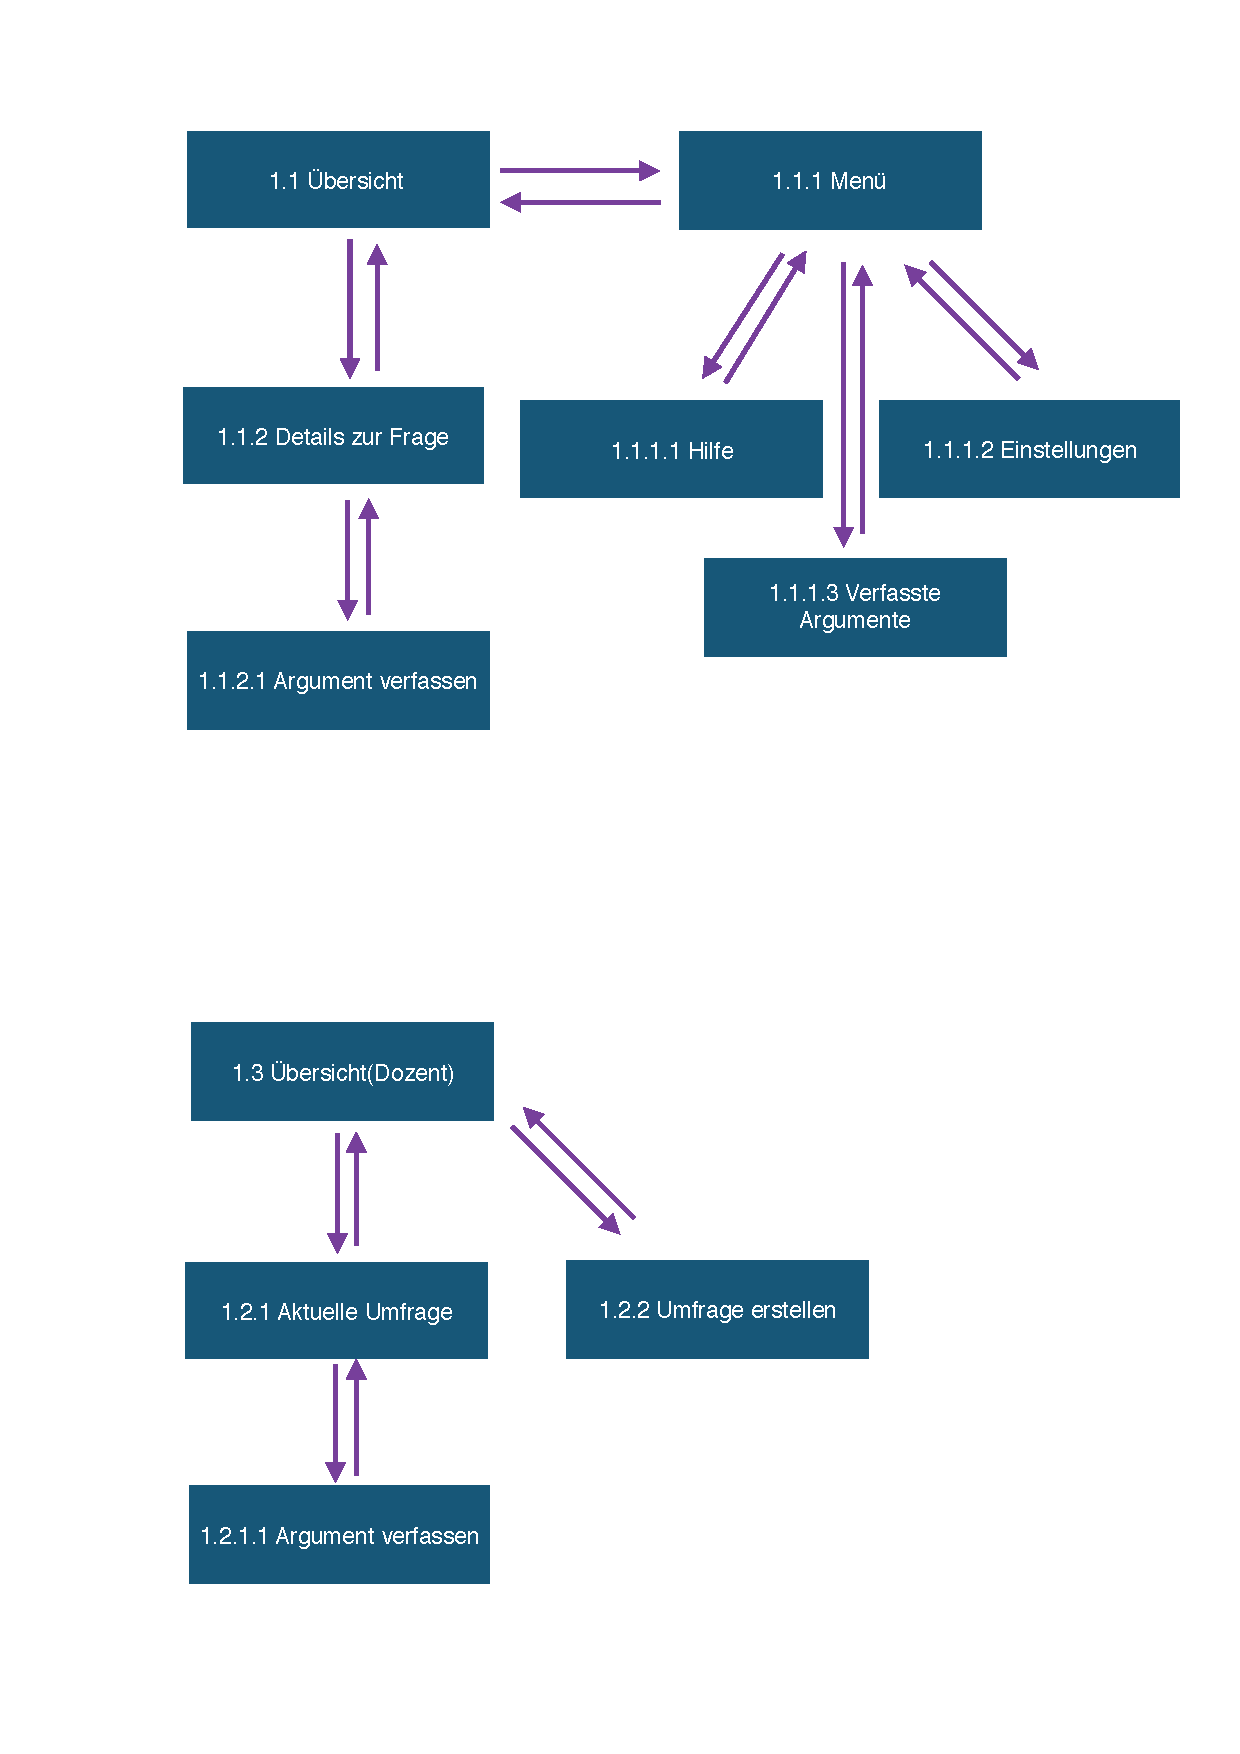
\includegraphics[page=1,width=0.79\textwidth]{./images/image}
  \end{center}
  \vspace{-40pt}
\end{wrapfigure}

\end{document}
